\documentclass[11pt,a4paper]{article}
\usepackage[T1]{fontenc}
\usepackage[utf8]{inputenc}
\usepackage{lmodern,microtype}
\usepackage[margin=24mm,top=23mm,bottom=24mm,headheight=15pt]{geometry}
\usepackage{amsmath,amssymb,amsthm,mathtools,booktabs,array,tabularx,longtable,enumitem,xcolor,fancyhdr,listings,tikz,float}
\usetikzlibrary{positioning,calc}
\definecolor{ink}{HTML}{17394A}
\definecolor{accent}{HTML}{126D71}
\definecolor{muted}{HTML}{53656D}
\definecolor{paperblue}{HTML}{EDF4F5}
\definecolor{falsecol}{HTML}{8C4236}
\usepackage[colorlinks=true,linkcolor=accent,citecolor=accent,urlcolor=accent,hypertexnames=false,
 pdfauthor={Keio and Shaitetsu},
 pdftitle={The Eighteen Conjectures of Fajtlowicz (1988): Truth Values, Proofs, and Counterexamples}]{hyperref}
\newtheorem{theorem}{Theorem}[section]
\newtheorem{lemma}[theorem]{Lemma}
\newtheorem{proposition}[theorem]{Proposition}
\newtheorem{corollary}[theorem]{Corollary}
\theoremstyle{remark}\newtheorem{remark}[theorem]{Remark}
\DeclareMathOperator{\dist}{dist}
\DeclareMathOperator{\diam}{diam}
\DeclareMathOperator{\rad}{rad}
\DeclareMathOperator{\supp}{supp}
\DeclareMathOperator{\rank}{rank}
\newcommand{\ad}{\operatorname{ad}}
\newcommand{\TRUE}{\textcolor{accent}{\textbf{True}}}
\newcommand{\FALSE}{\textcolor{falsecol}{\textbf{False}}}
\newcommand{\doi}[1]{\href{https://doi.org/#1}{doi:#1}}
\newcommand{\Ftwo}{\mathbb F_2}
\setlist{topsep=4pt,itemsep=3pt,parsep=0pt,leftmargin=*}
\setlength{\parindent}{1.1em}
\setlength{\parskip}{2pt}
\setlength{\emergencystretch}{3em}
\setlength{\tabcolsep}{5pt}
\renewcommand{\arraystretch}{1.14}
\pagestyle{fancy}\fancyhf{}
\fancyhead[L]{\small\color{muted}Fajtlowicz (1988): the eighteen conjectures}
\fancyhead[R]{\small\color{muted}Truth-status synthesis}
\fancyfoot[C]{\small\thepage}
\renewcommand{\headrulewidth}{0.3pt}
\raggedbottom
\lstset{language=Python,basicstyle=\ttfamily\scriptsize,columns=fullflexible,
 keepspaces=true,showstringspaces=false,breaklines=true,breakatwhitespace=false,
 frame=single,rulecolor=\color{muted!25},framesep=5pt,
 aboveskip=8pt,belowskip=8pt,tabsize=4}
\begin{document}
\thispagestyle{plain}
\noindent{\sffamily\small\bfseries\color{accent} GRAPH THEORY\quad /\quad SOURCE SYNTHESIS AND VERIFICATION}\par
\vspace{9pt}
\noindent{\LARGE\bfseries\color{ink}The Eighteen Conjectures\\[3pt]of Fajtlowicz (1988)}\par
\vspace{6pt}
\noindent{\large Truth Values, Proofs, and Counterexamples}\par
\vspace{8pt}
\noindent Keio and Shaitetsu\hfill 24 November 2026\par
\vspace{10pt}\hrule\vspace{10pt}
\noindent\textbf{Abstract.}
We determine the truth values of the eighteen statements printed under the heading
\emph{Open} on page 115 of Fajtlowicz's 1988 article \emph{On conjectures of Graffiti}.
The resulting classification is six true statements and twelve false statements.
The true entries are 1, 4, 11, 12, 13 and 14; all other entries are false.
We preserve the original numbering, specify the statistical conventions, and give
the correspondence with the later \emph{Written on the Wall} catalogue.
The account combines primary published results with the Verifiable Mathematical
Reasoning Corpus (VMRC), fixed at an identified revision. We reproduce the corpus
arguments for the radius and average-distance inequalities, including the
computation-free weighted-distance proof. All twelve negative verdicts have
explicit graph constructions and exact certificates; a complete standard-library
Python verifier is embedded in this single TeX source. The source labels distinguish
published literature from corpus arguments reproduced and examined here.

\section{Scope and principal conclusion}
The target is the \emph{first} numbered list of eighteen conjectures in
Fajtlowicz~\cite[p.~115]{fajtlowicz}. A separate list of twelve already-proved
statements follows in the same article. Those twelve statements are not part of
the present problem. The original article also has a note added in proof:
entries 1 and 14 were proved and entry 7 was refuted before publication
\cite[p.~118]{fajtlowicz}.

The domain is finite simple undirected graphs, with connectedness and at least
two vertices whenever distances are used. The inverse-degree sum requires no
isolated vertices. Every negative example in this paper is connected. The proof
of entry 1 also covers disconnected graphs, including edgeless graphs.

\begin{theorem}[Complete classification]\label{thm:classification}
With the definitions in Section~\ref{sec:notation}, the true entries in the
1988 list are exactly
\[
 \mathcal T=\{1,4,11,12,13,14\},
\]
and the false entries are exactly
\[
 \mathcal F=\{2,3,5,6,7,8,9,10,15,16,17,18\}.
\]
The affirmative claims in entries 11--13 use the corpus proofs reproduced in
Sections~\ref{sec:radius}--\ref{sec:weighted}; the negative claims are certified
in Sections~\ref{sec:counterexamples}--\ref{sec:rankcounter}.
\end{theorem}

The theorem is an integrated mathematical conclusion. The external literature
already supplies entries 1, 4 and 14 and several historical refutations.
The unrestricted radius and average-distance proofs used for entries 11--13
are corpus results, not claims of a newly located external journal publication.
Reproducing and checking their arguments does not by itself establish external
referee acceptance or historical priority.

\clearpage
\section{Definitions and the full ledger}\label{sec:notation}
Write $n=|V(G)|$, $d_v=\deg_G(v)$ and $A=A(G)$. Our notation is:
\begin{center}\small
\begin{tabularx}{\linewidth}{@{}lX@{}}\toprule
Symbol & Definition\\\midrule
$\mu$ & Average distance over distinct unordered pairs:
$\displaystyle\mu=\binom n2^{-1}\sum_{\{u,v\}}\dist(u,v)$.\\
$m$ & Most frequent positive distance; choose the largest distance in a tie.\\
$r,D$ & Vertex radius and diameter.\\
$R$ & $\displaystyle\sum_{uv\in E(G)}(d_ud_v)^{-1/2}$, the Randi\'c index.\\
$I$ & $\displaystyle\sum_{v\in V(G)}d_v^{-1}$, the inverse-degree sum.\\
$f$ & $\displaystyle\max_j|\{v:d_v=j\}|$, maximum degree multiplicity.\\
$z$ & $|\{v:d_v=\Delta\}|$, the number of maximum-degree vertices (``zenith'').\\
$\sigma^2$ & $\displaystyle n^{-1}\sum_vd_v^2-(n^{-1}\sum_vd_v)^2$,
the population variance of degrees.\\
$\tau$ & $\displaystyle n^{-1}\sum_v\frac{d_v}{n-d_v}$, average temperature.\\
$\alpha,\nu,\chi$ & Independence number, maximum matching size, chromatic number.\\
$q$ & $\rank_{\mathbb R} A(G)$.\\\bottomrule
\end{tabularx}
\end{center}

The mode $m$ is a distance value; $f$ is a multiplicity. They must not be
interchanged. The distance mean is not a mean over all $n^2$ matrix entries.
The degree variance uses denominator $n$, not $n-1$. These conventions are
those specified around the original list \cite[pp.~114--115]{fajtlowicz}.
The counterexamples involving $m$ have a unique mode, which is also unchanged
if ordered pairs and diagonal zeros are included.

\begin{center}\small
\begin{tabularx}{\linewidth}{@{}r l l X@{}}\toprule
1988 & Original proposed inequality & Verdict & Decisive evidence\\\midrule
1 & $\tau\le q$ & \TRUE & Elementary clique argument; original note in proof.\\
2 & $\tau\le\sigma^2+f$ & \FALSE & 12-vertex complement construction.\\
3 & $I\le R+f$ & \FALSE & 34-vertex bipartite certificate from VMRC [243].\\
4 & $m\le r+R$ & \TRUE & $m\le D\le r+R$, using the diameter theorem.\\
5 & $m\le\mu+R$ & \FALSE & 157-vertex tree, unique mode 113.\\
6 & $m\le\nu+\mu$ & \FALSE & The same tree, with $\nu=58$.\\
7 & $r\le z+f$ & \FALSE & Clique chain $A_1$, order 30.\\
8 & $r\le\sigma^2+f$ & \FALSE & Clique chain $A_3$, order 90.\\
9 & $r\le R+\tau$ & \FALSE & Even path $P_{26}$.\\
10 & $r\le R+\sigma^2$ & \FALSE & Even path $P_{22}$.\\
11 & $r\le\mu+R$ & \TRUE & Corpus radius bound and $\mu\ge1$.\\
12 & $r\le1+R$ & \TRUE & Corpus proof of $M\ge\rho\ge r-1/2$.\\
13 & $\mu\le R$ & \TRUE & VMRC [227] weighted-distance proof and transfer.\\
14 & $\mu\le\alpha$ & \TRUE & Chung's published theorem (1988).\\
15 & $\mu\le\sigma^2+f$ & \FALSE & Clique chain $A_{20}$, order 600.\\
16 & $\mu\le\sigma^2+I$ & \FALSE & Clique chain $B_{700}$, order 28,000.\\
17 & $\mu\le m+I$ & \FALSE & Clique chain $B_{100}$, order 4,000.\\
18 & $\chi\le1+q$ & \FALSE & Alon--Seymour graph: $\chi=32$, $q=29$.\\\bottomrule
\end{tabularx}
\end{center}
The auxiliary $M$ and absolute radius $\rho$ in row 12 are defined in
Section~\ref{sec:radius}. The graph families $A_p$ and $B_p$ are defined in
Section~\ref{sec:chains}. No minimal-order assertion is made for our witnesses.

\clearpage
\section{Numbering and source provenance}\label{sec:provenance}
The later catalogue changes the order of the questions. Table~\ref{tab:crosswalk}
records the correspondence to the July 2004 copy of \emph{Written on the Wall}
(WoW) \cite{wow}. The original article's full text was recovered from an
article mirror; its mathematical signs have imperfect OCR. We normalize the
inequalities to $\le$, corroborated by the author's verbal formulations for
the seventeen entries with catalogue counterparts. Entry 3 is false under
either a strict or a weak reading. The original page image was not available
for visual inspection.
\begin{table}[H]\centering\small
\begin{tabular}{@{}r r@{\qquad\qquad}r r@{}}\toprule
1988 & WoW (July 2004) & 1988 & WoW (July 2004)\\\midrule
1&10&10&15\\2&11&11&14\\3&---&12&12\\4&7&13&3\\
5&8&14&2\\6&9&15&6\\7&18&16&4\\8&17&17&5\\9&16&18&1\\\bottomrule
\end{tabular}
\caption{The original list and the later catalogue are not interchangeable.
The dash means that original entry 3 is absent from the first eighteen WoW entries.}
\label{tab:crosswalk}
\end{table}
In particular, WoW 13 is $r\le\mu+I$, a different statement; it must not
replace original entry 3. The label ``Fajtlowicz conjecture'' by itself is
insufficient to identify one of the many inequalities.

The author's catalogue records Staton's refutation of original entry 2
(June 1988), Qi's refutation of entry 6 (March 1990), Chen's refutation of
entry 7 (March 1988), and Shearer's refutations of entries 8 and 15
(October 1989). It also records the even-path failures of entries 9 and 10
associated with Caporossi and Hansen \cite[pp.~14--19]{wow}.
Our certificates below determine the truth values directly; these historical
annotations are not substitutes for an actual graph. Nor do we identify our
selected witnesses with the historical authors' unprinted examples.

\subsection{The fixed corpus revision}
The VMRC sources were read at revision
\begin{center}\small\ttfamily
52c1e4ae1f82bd3fdc8b809b9a94e2e4c6ef4cb3.
\end{center}
The relevant chain of sources is:
\begin{center}\small
\begin{tabularx}{\linewidth}{@{}lX@{}}\toprule
Corpus item & Role in this paper\\\midrule
{[161], [171]} & Original degree-cut arguments for the radius inequalities.\\
{[189]} & Earlier partial average-distance work; not the final global input.\\
{[226]} & Full proposed average-distance proof, with a finite core stage.\\
{[227]} & Subsequent hand proof of the weighted theorem, eliminating that enumeration.\\
{[243]} & The 34-vertex inverse-degree witness and periodic clique-chain method.\\
{[244]} & The modal-distance tree and a self-contained radius reconstruction.\\\bottomrule
\end{tabularx}
\end{center}
The precise filenames, frozen links and source hashes are recorded in
Appendix~\ref{app:manifest}. The earlier limited scope of [189] and the later
global claims of [226]--[227] describe successive stages, not two simultaneous
verdicts on the same proof. The proof used here for entry 13 is the
enumeration-free argument of [227].

Focused primary-source searches did not locate an unrestricted external journal
proof of entries 11--13. For example, Deng, Tang and Zhang's published radius
result \cite{deng} concerns trees and bounds involving the cyclomatic number;
it is not a general proof of original entry 12. The full proofs in the present
paper are therefore attributed to the corpus, with their arguments included.

\section{The affirmative entries supplied by the literature}\label{sec:externaltrue}
\subsection{Entry 1: average temperature versus adjacency rank}
The original note added in proof records this entry as proved by Fajtlowicz.
Here is an elementary verification that is independent of any rank-coloring
claim.
\begin{proposition}\label{prop:temperature}
For every nonempty graph with an edge,
\[
 \tau\le\omega(G)-1\le q-1.
\]
For an edgeless graph, $\tau=q=0$. In particular entry 1 is true.
\end{proposition}
\begin{proof}
The identity $d/(n-d)=n/(n-d)-1$ gives
$\tau+1=\sum_v1/(n-d_v)$. Choose a uniformly random ordering of the
vertices and retain $v$ when it precedes every other vertex not adjacent to it.
Two nonadjacent vertices cannot both be retained. The retained set is a
clique and its expected size is $\sum_v1/(n-d_v)$. Hence
$\tau+1\le\omega(G)$. If $\omega\ge2$, the adjacency matrix of a
maximum clique is a nonsingular principal submatrix of $A$, with eigenvalues
$\omega-1,-1,\ldots,-1$. Thus $\omega\le q$. The edgeless case is immediate.
\end{proof}

\subsection{Entry 4: modal distance versus radius and Randi\'c index}
Dvo\v{r}\'ak, Lidick\'y and \v{S}krekovski proved
$R(G)\ge D(G)/2$ for every connected graph \cite{dls}; their actual theorem
uses the smaller index $M=\sum_{uv}1/\max(d_u,d_v)$. The elementary bounds
$m\le D$ and $r\ge D/2$ therefore give
\[
 m\le D\le r+R.
\]
This settles entry 4. It does not justify replacing $r$ by $\mu$ in the
same formula: the resulting entry 5 has the explicit counterexample below.

\subsection{Entry 14: mean distance versus independence number}
Chung's theorem \cite{chung} states that every connected graph satisfies
\[
 \mu(G)\le\alpha(G).
\]
Its hypotheses and average-distance normalization agree with original
entry 14. The published theorem is the input here; no new proof or new
priority is claimed for it. The original article's note added in proof
also attributes this resolution to Chung \cite[p.~118]{fajtlowicz}.

\section{Explicit counterexamples}\label{sec:counterexamples}
\subsection{Entry 2: a twelve-vertex temperature example}
Let $G$ be the complement of the disjoint union $4K_1\sqcup2K_2\sqcup C_4$.
Its degrees $11,10,9$ each occur four times. In particular $G$ is connected,
and direct arithmetic gives
\[
 f=4,\qquad \sigma^2=\frac23,\qquad
 \tau=\frac1{12}\left(4\cdot11+4\cdot\frac{10}{2}
                         +4\cdot\frac93\right)=\frac{19}{3}.
\]
Thus $\tau=19/3>14/3=\sigma^2+f$, refuting entry 2.

\subsection{Entry 3: the thirty-four-vertex bipartite example}
Use two vertices $a,b$, sixteen leaves adjacent only to $a$, and sixteen
vertices adjacent to both $a$ and $b$. There is no edge $ab$.
This is the explicit construction in VMRC [243] \cite{vmrc243}.
The degrees are $32,16$, sixteen ones and sixteen twos. Consequently
\[
 I=16+8+\frac1{32}+\frac1{16}=\frac{771}{32},\quad
 f=16,\quad R=2+4\sqrt2.
\]
It follows that
\[
 I-(R+f)=\frac{195}{32}-4\sqrt2>0,
\]
where positivity follows by squaring the two positive terms:
$195^2>2\cdot128^2$. Thus entry 3 fails even on connected bipartite graphs.

\begin{figure}[ht]\centering
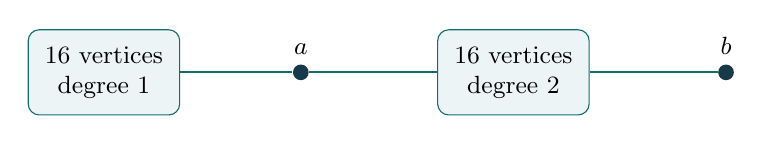
\begin{tikzpicture}[vertex/.style={circle,fill=ink,inner sep=2pt},
 group/.style={draw=accent,rounded corners,fill=paperblue,align=center,inner sep=6pt},
 every node/.style={font=\small}]
 \node[vertex,label=above:$a$] (a) at (0,0) {};
 \node[vertex,label=above:$b$] (b) at (5.4,0) {};
 \node[group] (leaf) at (-2.5,0) {16 vertices\\degree 1};
 \node[group] (common) at (2.7,0) {16 vertices\\degree 2};
 \draw[accent,thick] (leaf)--(a)--(common)--(b);
\end{tikzpicture}
\caption{The entry 3 witness. Each line to a box represents adjacency to
every vertex in that box; there are no other edges.}
\end{figure}

\subsection{Entries 5 and 6: a tree with unique distance mode 113}\label{sec:modetree}
Take the path $v_0,\ldots,v_{110}$. Add two vertices $a,b$ adjacent to
$v_0$, twelve new leaves at each of $a,b$, and twenty new leaves at
$v_{110}$. This is the 157-vertex tree of VMRC [244] \cite{vmrc244}.
\begin{figure}[ht]\centering
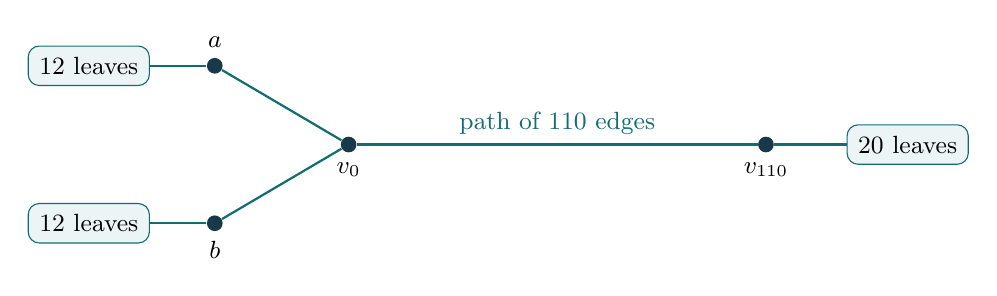
\begin{tikzpicture}[vertex/.style={circle,fill=ink,inner sep=2pt},
 group/.style={draw=accent,rounded corners,fill=paperblue,inner sep=4pt},
 every node/.style={font=\small}]
 \node[vertex,label=below:$v_0$] (v) at (0,0) {};
 \node[vertex,label=below:$v_{110}$] (w) at (5.3,0) {};
 \node[vertex,label=above:$a$] (a) at (-1.7,1) {};
 \node[vertex,label=below:$b$] (b) at (-1.7,-1) {};
 \node[group] (la) at (-3.3,1) {12 leaves};
 \node[group] (lb) at (-3.3,-1) {12 leaves};
 \node[group] (lc) at (7.1,0) {20 leaves};
 \draw[accent,thick] (a)--(v)--(b);
 \draw[accent,thick] (la)--(a) (lb)--(b) (w)--(lc);
 \draw[accent,thick] (v)--node[above]{path of 110 edges}(w);
\end{tikzpicture}
\caption{The same explicit tree refutes both modal-distance inequalities.}
\end{figure}

Let $h_j$ be the number of unordered vertex pairs at distance $j$.
Counting spine pairs, leaf--spine pairs and pairs in different leaf groups gives
\begin{equation}\label{eq:treehist}
\begin{array}{c|rrrrrrr}
j&1&2&3&4&5\le j\le111&112&113\\\hline
h_j&156&478&178&297&157-j&64&480.
\end{array}
\end{equation}
For example, $h_2=\sum_v\binom{d_v}{2}=478$ and the $480$ diametral
pairs join one of the 24 near leaves to one of the 20 remote leaves.
There are $\binom{157}{2}=12,246$ pairs in total. The largest frequency
is uniquely $480$, so $m=D=113$. The distance sum and mean are
\[
 W=\sum_j jh_j=576,558,\qquad
 \mu=\frac{96,093}{2,041}<47.09.
\]
The edge-degree products give
\begin{equation}\label{eq:treerandic}
 R=54+\frac1{\sqrt6}+\frac1{\sqrt{42}}+\frac2{\sqrt{39}}
                 +\frac{24}{\sqrt{13}}+\frac{20}{\sqrt{21}}<65.904.
\end{equation}
The strict upper bound is rationally certified by replacing each denominator
$\sqrt j$ with $\lfloor10^4\sqrt j\rfloor/10^4$; the five integer
floors are $24494,64807,62449,36055,45825$, respectively. Appendix
\ref{app:verifier} implements the same comparison with still finer integer
intervals. Therefore
\[
 \mu+R<112.994<113=m,
\]
which refutes entry 5.

For entry 6, delete $a,b,v_{110}$. The remaining nontrivial component is
the 110-vertex path $v_0,\ldots,v_{109}$, so any matching has size at most
$55+3=58$. A perfect matching of that path and one leaf edge at each of
the three deleted vertices attains 58. Thus
$\mu+\nu<47.09+58<113=m$. Both refutations remain valid with ordered
pairs, or with diagonal zeros included in the mode computation.

\subsection{Entries 9 and 10: even paths}
For $P_n$, $n\ge3$, direct evaluation gives
\[
 R=\frac{n-3}{2}+\sqrt2,\quad r=\lfloor n/2\rfloor,\quad
 \tau=\frac2{n-1},\quad \sigma^2=\frac{2(n-2)}{n^2}.
\]
At $n=26$,
\[
 r-(R+\tau)=\frac{71}{50}-\sqrt2>0,
\]
and at $n=22$,
\[
 r-(R+\sigma^2)=\frac{343}{242}-\sqrt2>0.
\]
Squaring verifies both strict inequalities. This refutes entries 9 and 10.
These even-path failures agree with the catalogue's recorded counterexample
families \cite{wow,caporossi}. The calculations also avoid confusing the
mean temperature with its unnormalized sum.

\section{Five refutations from two clique chains}\label{sec:chains}
Given positive integers $s_1,\ldots,s_L$, replace the successive vertices of
a path by cliques of these sizes and join consecutive cliques completely.
No edges join nonconsecutive layers. Denote the resulting connected graph
by $C(s_1,\ldots,s_L)$. This is the periodic clique-chain method used in
VMRC [243] \cite{vmrc243}; its relation to earlier inverse-degree
counterexamples is discussed in Erd\H{o}s, Pach and Spencer \cite{eps}.

Set $s_0=s_{L+1}=0$, $n=\sum_i s_i$ and $S_i=\sum_{j\le i}s_j$.
Every vertex in layer $i$ has degree
\[
 d_i=s_{i-1}+s_i+s_{i+1}-1.
\]
Two vertices in different layers $i,j$ are at distance $|i-j|$.
Vertices in one layer are at distance one. Therefore
\begin{align}
 I&=\sum_i\frac{s_i}{d_i},\quad
 \sigma^2=\frac{\sum_i s_i d_i^2}{n}
                 -\left(\frac{\sum_i s_i d_i}{n}\right)^2,\label{eq:chaindegree}\\
 W&=\sum_i\binom{s_i}{2}+\sum_{i=1}^{L-1}S_i(n-S_i),\label{eq:chainw}\\
 h_j&=\sum_{i=1}^{L-j}s_i s_{i+j}\quad(j\ge2),\qquad
 h_1=\sum_i\binom{s_i}{2}+\sum_{i=1}^{L-1}s_i s_{i+1}.\label{eq:chainhist}
\end{align}
The edge-cut sum in \eqref{eq:chainw} counts every cross-layer pair once
for each layer boundary between its endpoints. These formulas are exact,
not asymptotic estimates.

\subsection{A sixteen-layer profile: entries 7, 8 and 15}
Let $A_p$ be the clique chain whose layer list is $p$ repetitions of
\begin{equation}\label{eq:profilea}
 (1,1,1,3,5,2,4,1,2,3,1,1,2,1,1,1).
\end{equation}
This particular profile was selected in the present verification; no
historical novelty or minimality is asserted. Substitution into
\eqref{eq:chaindegree}--\eqref{eq:chainw} gives
\begin{align}
 n&=30p,& f&=5p,&z&=2p,&r&=8p,\label{eq:profileavalues}\\
 \sigma^2&=\frac{1499}{225}+\frac{127}{225p}-\frac1{225p^2},\label{eq:profileavar}\\
 W&=2400p^3-402p,&
 \mu&=\frac{800p^2-134}{5(30p-1)}.\label{eq:profileamean}
\end{align}
For an explicit degree check, the multiplicities at degrees
$1,2,3,4,5,6,8,9,10$ are respectively
\[
 2,\ 4p-2,\ 4p,\ 2p,\ 5p,\ 5p,\ 3p,\ 5p,\ 2p.
\]
The diameter is $16p-1$, giving the stated radius. These identities produce
three finite certificates:
\begin{center}\small
\begin{tabular}{@{}r r r l@{}}\toprule
Entry & $p$ & Order & Positive violation\\\midrule
7 &1&30& $r-z-f=8-2-5=1$\\
8 &3&90& $r-f-\sigma^2=24-15-13871/2025=4354/2025$\\
15&20&600& $\mu-f-\sigma^2=3287/30000$\\\bottomrule
\end{tabular}
\end{center}
For the last row, $\mu=534/5$ and $\sigma^2=200713/30000$.
Thus a degree-multiplicity correction does not rescue either the radius
or the average-distance bound.

\subsection{A four-layer profile: entries 16 and 17}
Let $B_p$ be the clique chain with $p$ repetitions of $(1,3,9,27)$.
The same elementary sums yield
\begin{align}
 n&=40p,&
 I&=\frac{362p}{285}+\frac9{28},\label{eq:profilebi}\\
 \sigma^2&=\frac{171}{4}+\frac{459}{20p}-\frac{729}{400p^2},\label{eq:profilebvar}\\
 W&=\frac{3200p^3-428p}{3},&
 \mu&=\frac{1600p^2-214}{30(40p-1)}.\label{eq:profilebmean}
\end{align}
For example, the degree multiplicities are
$3:1$, $12:3p$, $30:p-1$, $35:27$, $36:27(p-1)$ and $38:9p$.
This directly verifies the reciprocal and variance formulas.

At $p=700$, the graph has 28,000 vertices and the displayed rational
expressions satisfy
\[
 \mu>933,\qquad I<890,\qquad\sigma^2<43.
\]
Thus $\mu>I+\sigma^2$, refuting entry 16. The large order causes no
unverified search step: the graph and every needed invariant are given by
closed formulas.

For the mode, the first four positive-distance frequencies are
\[
 h_1=690p-27,\quad h_2=180p-90,\quad
 h_3=300p-273,\quad h_4=820(p-1).
\]
Periodicity makes $h_{j+4}<h_j$ whenever both bins exist: shifting by four
keeps every common summand and removes a positive tail. For $j=1$ the
within-layer terms only strengthen this comparison. If $p\ge7$, $h_4$
is strictly larger than each of $h_1,h_2,h_3$. Therefore $m=4$ uniquely.
At $p=100$, the graph has 4,000 vertices, $\mu>133$ and $I<128$.
It follows that $\mu>m+I$, refuting entry 17. Diagonal zeros also cannot
displace this mode, because $2h_4>n$.

\section{Entry 18: the Alon--Seymour graph}\label{sec:rankcounter}
The published counterexample of Alon and Seymour \cite{alon} refutes even
the original statement with its extra $+1$. An explicit certificate is short.
On $\Ftwo^6$, set $L=\{0,e_1,\ldots,e_6,(1,\ldots,1)\}$ and join
$x,y$ when $x+y\notin L$. Equivalently their Hamming distance is 2, 3, 4 or 5.
The graph has 64 vertices and degree 56, hence is connected.

The sum of any two distinct nonzero members of $L$ is outside $L$.
Consequently no independent triple exists. Pairing each vector with its
translate by $e_1$ partitions the graph into 32 independent pairs, so
$\chi=32$. For a Walsh character indexed by a vector of weight $j$, the
eigenvalue is 56 when $j=0$, and $2j-7-(-1)^j$ otherwise. Thus the spectrum is
\[
 56^{(1)},\quad(-4)^{(21)},\quad0^{(35)},\quad4^{(7)}.
\]
The adjacency rank is $q=29$, and $32>1+29$. Appendix~\ref{app:verifier}
checks the character equations, multiplicities and coloring with integers.

\section{The corpus radius proof: entries 12 and 11}\label{sec:radius}
Define the modified Randi\'c index
\[
 M(G)=\sum_{uv\in E(G)}\frac1{\max(d_u,d_v)}\le R(G).
\]
Give every edge length one. Let $\rho(G)$ be the minimum, over all points
of the resulting metric graph, of the maximum distance to its vertices.
This is an absolute center radius, not the vertex radius $r$.
A center is available at a vertex or an edge midpoint: along an edge,
distances to vertices are minima of affine functions with slopes $1,-1$
and integer intercepts, whose order changes only at half-integers.
The maximum distance is affine on each open half-edge. Rounding a center
to a nearest vertex proves
\begin{equation}\label{eq:absoluteradius}
 r-\frac12\le\rho\le r.
\end{equation}

The following degree-cut argument is reconstructed from VMRC
[161,171,244] \cite{vmrc161,vmrc171,vmrc244}. It is independent of the
average-distance theorem in the next section.
\begin{theorem}\label{thm:radius}
Every connected finite simple graph satisfies $M(G)\ge\rho(G)$.
Consequently $r\le R+1/2$, which proves original entry 12.
Since $\mu\ge1$, original entry 11 follows as well.
\end{theorem}
\begin{proof}
\emph{Tree facts.} A tree of diameter $D$ has absolute radius $D/2$:
at the position $i$ on a diameter path, each branch has depth at most
$\min(i,D-i)$, so its vertices lie within $D/2$ of the midpoint.
The ends give the reverse inequality. If a connected $m$-vertex graph
has a vertex incident to $j\ge2$ edges, extend these edges to a spanning
tree. Each of its $j$ branches there contains a different leaf. A longest
path uses at most two leaves, so the tree has diameter at most $m-j+1$.
Consequently the graph satisfies $2r\le m-j+2$.

\emph{Reduction to a core and its leaves.} Suppose $M<\rho$, and minimize
first the cycle rank $|E|-|V|+1$, then $|E|$. Deleting a nonbridge
edge cannot lower $\rho$: distances between retained points can only
increase, and possible center locations are lost. Hence every such deletion
strictly increases $M$ by minimality. Deletion of a leaf on a support
$v$ of degree $d\ge2$ decreases $M$ by
\[
 \frac1d-\frac{b}{d(d-1)}\ge0,
\]
where $b$ counts its other neighbors of degree less than $d$.
The deleted edge contributes $1/d$ and exactly those $b$ edges
increase in weight. This deletion can lower $\rho$ by at most $1/2$.
Indeed, take a vertex or midpoint center $y$ of the remaining graph of
radius $r_0$. If its distance to $v$ is at most $r_0-1/2$, restoration
already costs at most $1/2$. Otherwise that distance equals $r_0$
by half-integrality; move $y$ half a unit toward $v$. This is possible
when the remaining graph has at least two vertices, and covers every
vertex within $r_0+1/2$. Stars and paths are checked directly, including
the singleton and single edge. In a remaining counterexample a support
of degree two has a nonleaf as its other neighbor; here the decrease
of $M$ is $1/2$, contradicting minimality. Two leaves on one support
are also impossible. After removing one, choose a center off the other
pendant interval: projection to the support can only reduce all other
distances, and the remaining leaf is now at distance one, at most
the radius since two vertices remain at distance two. Restoring the
deleted twin costs nothing.

For every $v$, at most one component of $G-v$ contains an edge.
Otherwise split those components into two sides $A,B$, each containing
an edge, and let $G_A$ keep $A\cup\{v\}$ with a new leaf for every
lost neighbor of $v$; define $G_B$ symmetrically. Both graphs preserve
the degree of $v$. Their cycle ranks sum to the original and each
has fewer edges, so both satisfy the desired absolute-radius bound.
Their added leaves together account for exactly one unit of index:
$M(G_A)+M(G_B)=M(G)+1$. Write $r_i=\rho(G_i)$ for $i=A,B$.
Each side has an artificial leaf and a retained neighbor of $v$, so
$r_i\ge1$ and we may project any center on an artificial pendant
interval to $v$. Choose such retained centers $y_i$ and write
$s_i=d(y_i,v)\le r_i-1$ by the distance to an artificial leaf.
On the path from $y_A$ through $v$ to $y_B$, use signed distance
$u\in[-s_A,s_B]$ from $v$. The two sides are covered with radii
$r_A+s_A+u$ and $r_B+s_B-u$, respectively. Their point of intersection,
if on the interval, has value at most $r_A+r_B-1$.
Otherwise the endpoint minimizing the larger function gives radius
$r_A$ or $r_B$, also at most $r_A+r_B-1$. Thus
$\rho(G)\le r_A+r_B-1\le M(G)$, a contradiction.

A tree of diameter at least four violates this cut-vertex property at
the third vertex of a diametral path. A smaller-diameter tree having
at most one leaf per support is a path. Hence our graph contains a
cycle. Choose a maximal induced two-connected subgraph $K$ containing
one. An outside component meeting $K$ at two distinct vertices would
give an ear between them: after deleting any one vertex the union of
the ear with $K$ stays connected. Thus each outside component has a
unique attachment. Removing that attachment shows that the component
contains no edge, since $K$ with one vertex removed is connected and
has an edge. The outside vertices are therefore leaves, with at most
one at each vertex of $K$. Every edge of $K$ is a nonbridge.

\emph{Counting the edges between degree classes.} All degrees in the
next calculation refer to $G$. At a core vertex $v$ let $p_v$ indicate an
attached leaf, $l_v$ count all strictly lower-degree neighbors and put
\[
 g_v=d_v(d_v-1),\qquad
 a_v=l_v/g_v,\qquad b_v=(d_v-l_v)/g_v .
\]
Deleting a core edge $uv$ with $d_u<d_v$ changes $M$ by $a_u-b_v$:
the remaining edges to lower-degree neighbors gain $1/g_u$ or $1/g_v$,
and the removed edge had weight $1/d_v$. For $d_u=d_v=d$ the change is
$(l_u+l_v-d+1)/(d(d-1))$. Both changes must be strictly positive.
If $l_u=0$, then $u$ has no leaf. A higher-degree neighbor violates the
first formula, and an equal-degree neighbor has $l_v\le d_v-1$,
violating the second. Thus $l_v\ge1$. All full degrees at core vertices are at least
three, as a degree-two vertex has two nonleaf core neighbors. A core
vertex of smallest full degree must support a leaf. Removing all leaves
therefore gives a smaller graph $K$ and
\[
 0\le\delta:=M(G)-M(K)<\rho(G)-\rho(K)\le1 .
\]
The last bound uses the extension of any core center to all attached
leaves. If $\Delta=3$, then every core vertex has one lower-degree
neighbor, its leaf. Deleting any core edge gives change zero, a
contradiction. Hence $\Delta\ge4$.

For $3\le k<\Delta$, let $S$ be the core vertices of full degree at
most $k$, let $N_k$ count the core edges leaving $S$, and orient each
unequal-degree core edge from lower to higher. Denote by $I,F$ the
oriented edges inside and leaving $S$, and by $e_v$ the number of
equal-degree neighbors. At $v$ the indegree is $l_v-p_v$ and the
outdegree is $d_v-l_v-e_v$. Summing the identity
$(d_v-l_v)a_v=l_vb_v$ over $S$ gives
\[
 \sum_{v\in S}p_v b_v
  =\sum_{uv\in I}(a_u-b_v)+\sum_{uv\in F}a_u+\sum_{v\in S}e_v a_v.
\]
Delete only the leaves attached to $S$. The loss of $M$ is the left
side less $\sum_{uv\in Q}1/g_u$, where $Q$ consists of equal-degree
edges with a deleted leaf at each end. Indeed a strict edge changes its
weight only if its higher-degree end loses a leaf, in which case it gains
$1/g_v$ at that end. Its support loses $1/d_v$ and has $l_v-1$ such
core neighbors, leaving precisely $b_v$. An equal-degree edge gains
only when both ends lose leaves.
Each edge of $Q$ contributes $a_u+a_v\ge2/g_u$ to the final sum in the
display; the first sum is positive term by term. Deleting the remaining
leaves can only lower $M$ further. Thus
\[
 \delta\ge\sum_{uv\in F}a_u\ge \frac{N_k}{k(k-1)}.
\]

Write $h=|V(K)|$. On each edge the difference between the reciprocal
degree sum and twice its $M$-weight is $|1/d_u-1/d_v|$. Summing over
edges counts every vertex once in the reciprocal degree sum.
A core edge from degree $d$ to $e>d$ contributes
$\sum_{k=d}^{e-1}1/[k(k+1)]$. Subtract the leaf terms to obtain
\[
 h-2M=\sum_{k=3}^{\Delta-1}\frac{N_k}{k(k+1)}
          -\sum_{v\in K}\frac{p_v}{d_v}\le(\Delta-4)\delta\le\Delta-4.
\]
Here the removed leaf weights sum to at least $\delta$, as retained
edges only gain weight, and the first sum is at most
$\delta\sum_{k=3}^{\Delta-1}(k-1)/(k+1)\le(\Delta-3)\delta$.
A vertex of full degree $\Delta$ has at least $\Delta-1$ neighbors
in $K$. The spanning-tree construction gives a core tree of diameter
at most $h-\Delta+2$. Restoring the leaves increases its diameter by
at most two. Its midpoint yields $2\rho\le h-\Delta+4\le2M$, the
required contradiction.

\end{proof}
In particular, neither entry 11 nor entry 12 is inferred from
$\mu\le R$ alone. The radius proof supplies their own valid implication chain
$r\le\rho+1/2\le M+1/2\le R+1/2$.

\section{The corpus weighted-distance proof: entry 13}\label{sec:weighted}
The main ingredient is the optimized quadratic distance bound of VMRC [227]
\cite{vmrc227}, building on [226] \cite{vmrc226}. The diagonal value below
is part of the theorem, and is not the diagonal of the usual distance matrix.
For a probability vector $p$ on $V(G)$, put
\[
 K(x,x)=2,\qquad K(x,y)=\dist(x,y)\ (x\ne y),\qquad
 F(G)=\max_{p\ge0,\,\sum p_x=1}p^{\mathsf T}Kp.
\]
Compactness ensures that the maximum exists.
\begin{theorem}[Weighted-distance inequality]\label{thm:weighted}
Every connected finite simple graph of order at least two satisfies
\begin{equation}\tag{W}\label{weighted}
 F(G)\le M(G)+1.
\end{equation}
\end{theorem}
We reproduce the proof because this is the principal global input for
original entry 13. The argument closes all core orders by hand and does
not rely on the older small-graph enumeration.

For every $G$ in scope, $M\ge1$: the edges at a maximum-degree vertex contribute exactly one.
\subsection{The possible shape of a counterexample}
Suppose a graph violates \eqref{weighted}. Choose one minimizing first its order and then its size, and fix a maximizing vector $p$. A connected proper subgraph $J$ of order at least two containing the support of any maximizing vector must have $M(J)>M(G)$. Indeed the distances of its remaining pairs can only increase, and minimality gives $F(J)\le M(J)+1$. In particular
\begin{equation}
 M(G-e)>M(G)\quad\text{for every edge on a cycle.}\label{supportive}
\end{equation}
A star has $F\le2=M+1$. In a double star write $a,b$ for the masses on the two sets of leaves. Only pairs from opposite leaf sets have kernel entry above two, so $F\le2+2ab\le5/2$. The smaller number $l\ge1$ of leaves at a centre gives $M=1+l/(l+1)\ge3/2$.

For a vertex of degree at least two set $g_v=d_v(d_v-1)$ and let $\ell_v$ count its strictly lower-degree neighbours. Removing a leaf at $v$ decreases $M$ by
\begin{equation}
 b_v=(d_v-\ell_v)/g_v\ge0.\label{bleaf}
\end{equation}
The lost edge weighs $1/d_v$, and each of the other $\ell_v-1$ edges to a lower neighbour gains $1/g_v$. Thus a leaf in a minimal counterexample has positive mass for every maximizer.

We detail the cut-vertex step, since the diagonal convention matters here. If a cut vertex $v$ separates two nontrivial components, partition $G-v=A\sqcup B$ without crossing edges and with each side containing such a component. On side $A$ retain $v$ and replace its $d_B$ neighbours across the cut by $d_B$ new leaves; construct $G_B$ symmetrically. These padded graphs have fewer vertices or, in case of a tie, fewer edges, because the discarded side contains an edge. Old degrees are preserved and the new leaves give $M(G_A)+M(G_B)=M(G)+1$. Project $A$ identically to $G_A$ and send $B\cup\{v\}$ to a single new leaf; use the symmetric projection for $G_B$. The two projected kernel values sum to at least $K(x,y)+2$ for each pair. For a pair in one side the second value is two. For opposite sides the two new terminal edges add two. For $v$ paired with another vertex the surplus is three, and for $(v,v)$ it is two. Taking expectations contradicts minimality. Hence at most one component of $G-v$ can be nontrivial.

Remove all leaves and denote the remaining graph by $J$. It is connected; the one- and two-vertex possibilities were covered above. A cut vertex of $J$ would leave two components of the original graph containing non-leaf vertices, each nontrivial, contrary to the preceding paragraph. Thus $J$ is two-connected of order $h\ge3$. Two leaves at the same site have identical rows on the other vertices, and their $2\times2$ kernel is constant. Merging their masses would give a zero-mass leaf. Consequently each site $v$ in $J$ has at most one leaf $v'$. Call it \emph{loaded} when it has one, and set $\epsilon_v=1$ there and $0$ elsewhere. All core edges obey \eqref{supportive}. Moving the entire mass $t=p_v$ of a loaded site to its leaf increases the objective by $2t(1-t)$, because all other distances go up by one and the diagonal is two. The case $t=1$ gives $F=2$. Thus $p_v=0$ at every loaded site.
\subsection{Degree restrictions and local deletion}
Put $a_v=\ell_v/g_v$, and use \eqref{bleaf} to define $b_v$ at every site. Deleting a core edge $uv$ gains $1/g_u$ on each surviving lower edge at $u$, and similarly at $v$, and loses its original weight. Hence \eqref{supportive} gives
\[
 d_u<d_v\Longrightarrow a_u>b_v,\qquad
 d_u=d_v\Longrightarrow a_u\ge b_v,\quad a_v\ge b_u .
\]
In the equal-degree case the strict inequality in the count is $\ell_u+\ell_v>d_u-1$, so the weak bounds follow by integrality. A site with no lower neighbour would contradict the first relation on a rising edge, or force $b_v=0$ on an equal edge where $u$ itself is not lower. A minimum-degree site therefore has a leaf and at least two core neighbours. Every site has total degree at least three. Every degree-three site is loaded, has exactly two core neighbours, and both have degree at least four by the equal-degree condition. This also rules out $h=3$.

Delete a site and its leaf if present, and denote the decrease of $M$ by $X_v$. The remaining graph is connected and has at least two vertices. Define
\[
 \beta_v=\epsilon_v b_v,\qquad \xi_v=\max(0,X_v,\beta_v).
\]
Every survivor edge can only grow in weight, while removed edges have total weight at most one. Thus $X_v\le1$. We need the following sharper bound.
\begin{lemma}\label{local}
At each site $0\le\beta_v\le\min(\xi_v,1/3)$ and $\xi_v+\beta_v\le1$.
\end{lemma}
\begin{proof}
Only a loaded site needs attention. Set $d=d_v$, $g=d(d-1)$, and let $l,e,u$ count its lower, equal and higher core neighbours. Then $l+e+u=d-1$ and $b_v=(e+u)/g\le1/d$. For a core neighbour $w$, its contribution to $X_v$ after subtracting survivor gains on its lower edges is $b_w$ if $d_w>d$, $b_w-1/g$ if $d_w=d$, and $1/d-a_w$ if $d_w<d$. If two equal-degree neighbours of $v$ are adjacent, the edge between them also gains, requiring a further subtraction. Dropping these nonnegative corrections gives an upper bound. The three preceding contributions are at most $a_v$, $a_v-1/g$ and $1/d-b_v$, respectively. Including the leaf edge gives
\[
 g X_v\le(d-1)+u(l+1)+el+l(d-1-e-u)=(l+1)(d-1)+u.
\]
Adding $gb_v=e+u$ leaves a shortfall from $g$ of $(d-2)e+(d-3)u\ge0$. Thus $X_v+b_v\le1$ and $2b_v\le2/3$, proving the claim.
\end{proof}
\subsection{The probability constraint}
For $u\in\supp p$, a one-sided transfer of mass from $u$ to any $z$ shows $(Kp)_u\ge(Kp)_z$. Averaging on the support yields $(Kp)_u=F(G)$. Suppose $S$ is a set whose deletion leaves a connected graph of order at least two, and only $u\in S$ may have positive mass. Set $t=p_u$, $x=M(G)-M(G-S)$ and $F=F(G)$. If $t=0$, then $x<0$ by the subgraph argument. For $0<t<1$, renormalize the surviving vector by $1-t$. The kernels of surviving pairs can only rise and $\sum_{z\ne u}p_z\dist(u,z)=F-2t$, whence
\[
 (1-2t)F\le (1-t)^2(M+1-x)-2t^2 .
\]
For $0<t<1/2$, using $F>M+1$ on the left gives $(1-t)^2x<(M-1)t^2$.

To justify the other half of the mass range, $M\ge2$ here: order the sites by decreasing degree and charge each edge to its first endpoint, putting leaves last. The first four sites contribute at least $\sum_{i=1}^4(1-(i-1)/3)=2$. Write $y=\sqrt{M-1}\ge1$ and $\theta(s)=\sqrt s/(y+\sqrt s)$. If $0<x\le1$, the last inequality gives $t>\theta(x)$ when $t<1/2$, and $\theta(x)\le1/2\le t$ otherwise. An unloaded site supplies mass for the deletion $\{v\}$. A loaded site supplies the same leaf mass for each of $\{v'\}$ and $\{v,v'\}$ because $p_v=0$. Summing these lower bounds over distinct masses yields
\begin{equation}
 \Theta:=\sum_{v\in V(J)}\theta(\xi_v)\le1.\label{budget}
\end{equation}

\subsection{Closing the weighted inequality}\label{sec:hand}
\begin{lemma}\label{saved}
Let $l_v$ count the lower \emph{core} neighbours of $v$, and $M_0$ be the weight of the core edges. Then
\[
 \sum_v X_v\ \ge\ M_0+\sum_{v\ \mathrm{loaded}}\frac{l_v}{g_v},
 \qquad M\le\sum_v(\xi_v+\beta_v).
\]
\end{lemma}
\begin{proof}
Sum the weight removed under site deletions. It is $2M_0+\sum_{v\ \mathrm{loaded}}1/d_v$ before the gains of surviving edges are subtracted. Each leaf edge at $w$ gains $1/g_w$ exactly $d_w-1$ times. For a core edge $uw$ with $d_u<d_w$, the gain $1/g_w$ occurs exactly when a core neighbour of $w$ other than $u$ is deleted. This is $d_w-1-\epsilon_w$ times, giving total $1/d_w-\epsilon_w/g_w$. On an equal-degree edge of degree $d$, gains occur only when a common neighbour is deleted, at most $d-1$ times, for total at most $1/d$. Subtract these gains. The unequal-degree term saves $1/g_w$ once for each lower core neighbour of a loaded $w$. Finally $1/d_v-l_v/g_v=b_v$ on a loaded site, since $\ell_v=l_v+1$. Adding the leaf weights to $M_0$ and using $X_v\le\xi_v$ proves the second claim.
\end{proof}
For a site with $x=\xi_v>0$, $b=\beta_v$, Lemma~\ref{local} gives $b\le x\le1-b$. The function $\sqrt{x}+b/\sqrt{x}$ is increasing on $x\ge b$, so
\[
 \frac{x+b}{\theta(x)}
   =(x+b)+y\bigl(\sqrt{x}+b/\sqrt{x}\bigr)
   \le1+\frac{y}{\sqrt{1-b}}\le1+\sqrt{3/2}\,y .
\]
At $x=0$ both summands in $x+b$ vanish. Lemma~\ref{saved} and \eqref{budget} now force $1+y^2=M\le1+\sqrt{3/2}\,y$, or
\begin{equation}M\le 5/2.\label{fivehalf}\end{equation}
\begin{lemma} If $h\ge5$, every surviving decorated core has $M>5/2$.\end{lemma}
\begin{proof}
Let $r$ be the number of sites of degree at least four. If some sites have degree three, each has two distinct higher neighbours, so $r\ge2$. For $2\le r\le4$, charge edges at the first endpoint in decreasing order. The first $r$ sites contribute at least $r-\binom r2/4$. Each remaining site contributes a separate leaf edge of weight $1/3$. At $h=5$ these lower bounds for $r=2,3,4$ are $11/4,35/12,17/6$. They increase with $h$. If $r\ge5$, the first five sites alone contribute at least $5-10/4=5/2$. For $h>5$ choose the last site in this ordering. Its lower neighbour must be a leaf, and that edge was uncounted. For $h=5$, a missing pair among the five gives strictness in counting earlier neighbours. If the core is $K_5$, an unloaded site would have degree four and no lower neighbour. All sites are therefore loaded and $M=3$.
\end{proof}
It remains to handle $h=4$. Every site has core degree at least two, so the missing pairs of $J$ form a matching. Project a leaf to its site and each site to itself, and write $q$ for the resulting masses. For independent samples $x,y$ from $p$, $K(x,y)\le2+\dist_J(\pi x,\pi y)$ even on the diagonal. Missing pairs have distance two, and hence
\[
 \mathbb E_q\dist_J
 =1-\sum_i q_i^2+2\sum_{ij\ \mathrm{missing}}q_iq_j\le1
\]
by $2q_iq_j\le q_i^2+q_j^2$ on disjoint pairs. Thus $F\le3\le M+1$. This contradicts minimality in the last possible case and proves \eqref{weighted}. In particular, no external computation is needed for this proof of the weighted theorem.


\subsection{Transfer from the quadratic bound to the ordinary mean}\label{sec:transfer}
Uniform mass on the vertices in (W) gives
\begin{equation}\label{eq:uniform}
 M\ge\frac{(n-1)\mu-(n-2)}n.
\end{equation}
Indeed the off-diagonal contribution is $(n-1)\mu/n$, while the diagonal
contributes $2/n$. Let $s=\sqrt\Delta$. For an edge with degrees $a\le b$,
\[
 \frac1a+\frac1b
 =\frac2{\sqrt{ab}}+
   \left(\sqrt{\frac ba}-1\right)
   \left(\frac1{\sqrt{ab}}-\frac1b\right).
\]
Since $\sqrt{b/a}-1\le s-1$, summation gives
\begin{equation}\label{eq:bridge}
 (s+1)R\ge n+(s-1)M.
\end{equation}
The left incidence sum is $n$, since a vertex of degree $d$ contributes
$d$ copies of $1/d$.

\begin{lemma}[The path upper bound]\label{lem:pathmean}
Every connected $n$-vertex graph satisfies $\mu\le(n+1)/3$, with equality
only for the path $P_n$.
\end{lemma}
\begin{proof}
Passing to a spanning tree cannot decrease any distance. For a leaf of
a tree of order $t$, sort its distances to other vertices as
$b_1\le\cdots\le b_{t-1}$. Then $b_i\le i$, because a path to distance
$k$ contains every smaller positive distance. Deleting a leaf therefore
removes at most $t(t-1)/2$ from the unordered distance sum. Induction gives
$W\le(n^3-n)/6$. Equality in the leaf transmission bound requires one
vertex at each distance and hence a path. An additional edge in a graph
strictly shortens the distance between its endpoints relative to the tree.
\end{proof}

\begin{theorem}[Original entry 13]\label{thm:meanrandic}
For every connected graph of order at least two, $\mu\le R$.
Equality holds precisely for $K_2$.
\end{theorem}
\begin{proof}
Suppose first that $n\ge5$ and $R\le\mu$. Combining
\eqref{eq:uniform} and \eqref{eq:bridge} gives
\[
 \mu\ge T(n,s):=\frac{n^2-(s-1)(n-2)}{2n+s-1}.
\]
For fixed $n>2$ this is strictly decreasing in $s$. Since
$s\le\sqrt{n-1}$, it remains to compare $T(n,\sqrt{n-1})$ with
$(n+1)/3$. After multiplying by positive denominators, the comparison is
\[
 n^2+2n-5\ \ge\ (4n-5)\sqrt{n-1}.
\]
Both sides are positive and their squared difference factors exactly as
\[
 (n^2+2n-5)^2-(4n-5)^2(n-1)
 =(n-5)(n-2)(n^2-5n+5).
\]
It is positive for $n>5$, contradicting Lemma~\ref{lem:pathmean}.
At $n=5$, equality throughout requires both $G=P_5$ and $\Delta=4$,
which is impossible.

For $n=3,4$, use $M\ge1$ in \eqref{eq:bridge}:
\[
 R\ge1+\frac{n-2}{\sqrt\Delta+1}
   \ge\sqrt{n-1}>\frac{n+1}{3}\ge\mu.
\]
The sole connected graph on two vertices is $K_2$, with $R=\mu=1$.
This completes the proof without graph enumeration.
\end{proof}

\section{What is established and how it was checked}\label{sec:verification}
The six affirmative verdicts have unrestricted graph scope under the
definitions stated above. Entries 1, 4 and 14 are supported by the primary
literature; entry 1 additionally has a self-contained proof here. Entries
11--13 are supported by the reproduced corpus arguments. The radius argument
and the weighted-distance argument were separately read and algebraically
rederived in this preparation. In particular, the degree-cut correction for
simultaneously removed leaves, the cut-vertex gluing bound, the probability
budget, and the last four-core-vertex case were examined explicitly.

Every negative verdict has a concrete graph. For the small explicit graphs,
independent breadth-first searches recompute all distances. Randi\'c sums
are enclosed by rational intervals obtained from integer square roots.
The clique chains are checked from the layer-degree and boundary-cut formulas;
this is exact compression of a specified finite graph, not sampling. The
rank-coloring graph is checked through its integer Walsh eigenbasis and
an explicit partition into independent pairs. The verifier was executed
successfully for all twelve negative entries.

These computational checks certify the displayed counterexamples; the
universal positive results rely on their proofs. The present work does not
claim a Lean or Coq verification, an external referee decision, or first
discovery of every proof or witness. Its conclusion is the complete
source-attributed classification in Theorem~\ref{thm:classification}.

\clearpage
\appendix
\section{Exact corpus source manifest}\label{app:manifest}
All links below refer to the same frozen commit printed in
Section~\ref{sec:provenance}; a moving branch name is not needed to reproduce
the source selection. The four principal source hashes are included to
disambiguate later revisions.
\begin{description}[font=\normalfont\bfseries]
\item[[161]] \href{https://github.com/QEEDDD/Verifiable-Mathematical-Reasoning-Corpus/blob/52c1e4ae1f82bd3fdc8b809b9a94e2e4c6ef4cb3/\%5B161\%5D\%20Randic\_Index\_and\_Vertex\_Radius.tex}{\nolinkurl{Randic_Index_and_Vertex_Radius.tex}}
\item[[171]] \href{https://github.com/QEEDDD/Verifiable-Mathematical-Reasoning-Corpus/blob/52c1e4ae1f82bd3fdc8b809b9a94e2e4c6ef4cb3/\%5B171\%5D\%20Harmonic\_Radius\_Master\_Theorem.tex}{\nolinkurl{Harmonic_Radius_Master_Theorem.tex}}
\item[[189]] \href{https://github.com/QEEDDD/Verifiable-Mathematical-Reasoning-Corpus/blob/52c1e4ae1f82bd3fdc8b809b9a94e2e4c6ef4cb3/\%5B189\%5D\%20Collected\_Research\_Papers.tex}{\nolinkurl{Collected_Research_Papers.tex}}
\item[[226]] \href{https://github.com/QEEDDD/Verifiable-Mathematical-Reasoning-Corpus/blob/52c1e4ae1f82bd3fdc8b809b9a94e2e4c6ef4cb3/\%5B226\%5D\%20Fajtlowicz\_Average\_Distance\_Proof.tex}{\nolinkurl{Fajtlowicz_Average_Distance_Proof.tex}}
\item[[227]] \href{https://github.com/QEEDDD/Verifiable-Mathematical-Reasoning-Corpus/blob/52c1e4ae1f82bd3fdc8b809b9a94e2e4c6ef4cb3/\%5B227\%5D\%20Fajtlowicz\_Proof\_Audit.tex}{\nolinkurl{Fajtlowicz_Proof_Audit.tex}}
\item[[243]] \href{https://github.com/QEEDDD/Verifiable-Mathematical-Reasoning-Corpus/blob/52c1e4ae1f82bd3fdc8b809b9a94e2e4c6ef4cb3/\%5B243\%5D\%20Graffiti\_Degree\_Multiplicity\_and\_Distance.tex}{\nolinkurl{Graffiti_Degree_Multiplicity_and_Distance.tex}}
\item[[244]] \href{https://github.com/QEEDDD/Verifiable-Mathematical-Reasoning-Corpus/blob/52c1e4ae1f82bd3fdc8b809b9a94e2e4c6ef4cb3/\%5B244\%5D\%20Graph\_Distance\_Modes\_and\_Extrema.tex}{\nolinkurl{Graph_Distance_Modes_and_Extrema.tex}}
\end{description}
\smallskip\noindent SHA-256 of the principal TeX sources:\par
\noindent [226] \texttt{34501109e2caf974b3f4765b2a649798}\\\hspace*{2.7em}\texttt{76d2b7cdcbf56648f0af42001c7f1335}\par
\noindent [227] \texttt{31b9760bf4f0436f333e96ea3a190ef8}\\\hspace*{2.7em}\texttt{cd22116e3297b49cd0e2dd676fd64361}\par
\noindent [243] \texttt{be93332b36b99f8e76fe4e1a3b4ed6f4}\\\hspace*{2.7em}\texttt{d2dc104d47ff767cde5a07ae4277de5b}\par
\noindent [244] \texttt{7c3b342c8917ebd49520d85b3c3df4a1}\\\hspace*{2.7em}\texttt{0d372b08564cddc2584ddc419fb15773}\par

\section{Complete exact-arithmetic verifier}\label{app:verifier}
Copy the following listing into a Python file and run it with Python 3.10 or
later, with assertions enabled. Only the standard library is required.
The code prints exact invariant values and ends with a success message for
all twelve false entries. It is included verbatim in this single TeX file;
no external code file or graph database is needed. The positive theorem proofs
do not depend on this program.
\begin{lstlisting}
#!/usr/bin/env python3
"""Independent exact certificates for false entries in Fajtlowicz's 1988 list.
Only the Python standard library is required. Graphs are simple, undirected,
and connected; mean distances use unordered distinct pairs. Largest mode wins.
Square-root expressions are bounded by rational intervals using integer sqrt.
"""
from collections import Counter, deque
from fractions import Fraction as Q
from math import isqrt
import json


def graph(n, edges):
    adj = [set() for _ in range(n)]
    for a, b in edges:
        assert a != b
        adj[a].add(b); adj[b].add(a)
    return adj


def path(n):
    return graph(n, ((i, i+1) for i in range(n-1)))


def mean_variance(adj):
    n = len(adj); ds = [len(a) for a in adj]
    return Q(sum(ds), n), Q(sum(d*d for d in ds), n)-Q(sum(ds), n)**2


def randic_interval(adj, scale=10**8):
    ds = [len(a) for a in adj]
    counts = Counter(ds[u]*ds[v] for u,a in enumerate(adj) for v in a if u<v)
    lo = hi = Q(0)
    for prod, mult in counts.items():
        a = isqrt(prod*scale*scale)
        hi += Q(mult*scale, a)
        lo += Q(mult*scale, a if a*a == prod*scale*scale else a+1)
    return lo, hi, counts


def invariants(adj):
    n = len(adj); ds = [len(a) for a in adj]
    assert min(ds)>0
    hist = Counter(); ecc = []
    for u in range(n):
        dist = [-1]*n; dist[u]=0; q=deque([u])
        while q:
            v=q.popleft()
            for w in adj[v]:
                if dist[w]<0:
                    dist[w]=dist[v]+1; q.append(w)
        assert min(dist)>=0
        ecc.append(max(dist))
        hist.update(dist[v] for v in range(u+1,n))
    assert sum(hist.values()) == n*(n-1)//2
    deg=Counter(ds)
    lo,hi,edge_products=randic_interval(adj)
    W=sum(k*v for k,v in hist.items())
    return dict(n=n, degree_histogram=deg, I=sum((Q(1,d) for d in ds),Q(0)),
                F=max(deg.values()),Z=deg[max(ds)], V=mean_variance(adj)[1],
                T=sum((Q(d,n-d) for d in ds),Q(0))/n,
                Rlo=lo,Rhi=hi,R_products=edge_products,
                r=min(ecc),D=max(ecc),mu=Q(W,n*(n-1)//2),W=W,
                mode=max(hist,key=lambda d:(hist[d],d)),histogram=hist)


def tree_matching(adj):
    root=0; parent=[-1]*len(adj); parent[root]=root; order=[root]
    for v in order:
        for w in adj[v]:
            if w!=parent[v]:
                assert parent[w]==-1
                parent[w]=v; order.append(w)
    A=[0]*len(adj);B=[0]*len(adj)
    for v in reversed(order):
        kids=[w for w in adj[v] if parent[w]==v and w!=v]
        A[v]=sum(B[w] for w in kids)
        B[v]=A[v]+max([0]+[1+A[w]-B[w] for w in kids])
    return B[root]


def complement_witness():
    # Complement of 4K1 + 2K2 + C4.
    absent={(4,5),(6,7),(8,9),(9,10),(10,11),(8,11)}
    return graph(12, ((i,j) for i in range(12) for j in range(i+1,12)
                      if (i,j) not in absent))


def inverse_degree_witness():
    # 0=a, 1=b; 16 a-only leaves, 16 vertices joined to both a,b.
    return graph(34, [(0,j) for j in range(2,34)]+[(1,j) for j in range(18,34)])


def mode_tree(L=110,near=12,far=20):
    edges=[(j,j+1) for j in range(L)]
    edges += [(0,L+1),(0,L+2)]
    nxt=L+3
    for hub, amount in [(L+1,near),(L+2,near),(L,far)]:
        edges += [(hub,j) for j in range(nxt,nxt+amount)]
        nxt+=amount
    return graph(nxt,edges)


def clique_chain(profile,p):
    """Compressed exact computation, not numerical or sampled graph search.
    Adjacent layers are completely joined, and every layer is a clique.
    h[d+K] < h[d] for d>=1 since the profile is K-periodic; for d=1
    there is the additional nonnegative within-layer term. Thus the largest
    modal distance lies among 1,...,K, and these bins suffice exactly.
    """
    ss=profile*p; K=len(profile);n=sum(ss);L=len(ss)
    dd=[ss[i]-1+(ss[i-1] if i else 0)+(ss[i+1] if i+1<L else 0) for i in range(L)]
    hist=Counter()
    for s,d in zip(ss,dd):hist[d]+=s
    S=0;W=sum(s*(s-1)//2 for s in ss)
    for s in ss[:-1]:
        S+=s;W+=S*(n-S)
    h={d:sum(ss[i]*ss[i+d] for i in range(L-d)) for d in range(1,K+1)}
    h[1]+=sum(s*(s-1)//2 for s in ss)
    I=sum((Q(s,d) for s,d in zip(ss,dd)),Q(0))
    mean=Q(sum(s*d for s,d in zip(ss,dd)),n)
    V=Q(sum(s*d*d for s,d in zip(ss,dd)),n)-mean*mean
    return dict(n=n,layers=L,F=max(hist.values()),Z=hist[max(hist)],
                degree_histogram=hist,I=I,V=V,r=L//2,D=L-1,
                W=W,mu=Q(W,n*(n-1)//2),mode=max(h,key=lambda d:(h[d],d)),
                first_period_distance_counts=h)


def summary(v):
    return {k:str(v[k]) for k in ['n','F','Z','I','V','r','D','W','mu','mode'] if k in v}


def main():
    report={}
    v=invariants(complement_witness())
    assert v['T']==Q(19,3) and v['V']==Q(2,3) and v['F']==4
    assert v['T']>v['V']+v['F']
    report['2']={**summary(v),'T':str(v['T'])}

    v=invariants(inverse_degree_witness())
    assert v['I']==Q(771,32) and v['F']==16
    assert v['I']>v['Rhi']+v['F']
    report['3']={**summary(v),'R_upper':str(v['Rhi']),
                 'edge_degree_products':str(v['R_products'])}

    adj=mode_tree();v=invariants(adj);nu=tree_matching(adj)
    assert v['n']==157 and v['W']==576558 and v['mu']==Q(96093,2041)
    assert v['mode']==113 and v['histogram'][113]==480
    assert max(c for k,c in v['histogram'].items() if k!=113)==478
    assert v['Rhi']<Q(65904,1000)
    assert v['mode']>v['mu']+v['Rhi']
    assert nu==58 and v['mode']>v['mu']+nu
    report['5,6']={**summary(v),'matching':nu,'R_upper':str(v['Rhi']),
                  'histogram_top5':v['histogram'].most_common(5)}

    motif=[1,1,1,3,5,2,4,1,2,3,1,1,2,1,1,1]
    for label,p in [('7',1),('8',3),('15',20)]:
        v=clique_chain(motif,p)
        assert v['n']==30*p and v['F']==5*p and v['Z']==2*p and v['r']==8*p
        assert v['W']==2400*p**3-402*p
        if label=='7': assert v['r']>v['Z']+v['F']
        if label=='8': assert v['r']>v['V']+v['F']
        if label=='15':
            assert v['mu']==Q(534,5) and v['V']==Q(200713,30000)
            assert v['mu']-v['F']-v['V']==Q(3287,30000)
        report[label]=summary(v)

    v=invariants(path(26))
    assert v['r']==13 and v['T']==Q(2,25)
    assert v['r']>v['Rhi']+v['T']
    report['9']={**summary(v),'T':str(v['T']),'R_upper':str(v['Rhi'])}

    v=invariants(path(22))
    assert v['r']==11 and v['V']==Q(10,121)
    assert v['r']>v['Rhi']+v['V']
    report['10']={**summary(v),'R_upper':str(v['Rhi'])}

    for label,p in [('16',700),('17',100)]:
        v=clique_chain([1,3,9,27],p)
        assert v['n']==40*p and v['W']==(3200*p**3-428*p)//3
        assert v['I']==Q(362*p,285)+Q(9,28)
        assert v['V']==Q(171,4)+Q(459,20*p)-Q(729,400*p*p)
        assert v['mode']==4
        if label=='16':
            assert v['mu']>933 and v['I']<890 and v['V']<43
            assert v['mu']>v['I']+v['V']
        else:
            assert v['mu']>133 and v['I']<128
            assert v['mu']>v['I']+v['mode']
        # Ordered distance matrix, even including diagonal zeros, still has mode4.
        assert 2*v['first_period_distance_counts'][4]>v['n']
        report[label]=summary(v)
    # Alon--Seymour 64-vertex Cayley graph; an exact Walsh certificate.
    nonzero_L={1,2,4,8,16,32,63}
    forbidden=nonzero_L|{0}
    allowed=set(range(64))-forbidden
    assert len(allowed)==56
    sign=lambda a,x: -1 if (a&x).bit_count()%2 else 1
    eigenvalues={a:sum(sign(a,s) for s in allowed) for a in range(64)}
    spectrum=Counter(eigenvalues.values())
    assert spectrum==Counter({56:1,-4:21,0:35,4:7})
    rank=sum(value!=0 for value in eigenvalues.values())
    assert rank==29
    # Walsh vectors form an orthogonal basis, and are adjacency eigenvectors.
    for a in range(64):
        for b in range(a,64):
            assert sum(sign(a,x)*sign(b,x) for x in range(64))==(64 if a==b else 0)
        for x in range(64):
            assert sum(sign(a,x^s) for s in allowed)==eigenvalues[a]*sign(a,x)
    # Three independent vertices translate to 0,a,b with a,b,a^b in L\{0}.
    # Distinct nonzero elements of L never have their XOR in L.
    assert all((a^b) not in nonzero_L for a in nonzero_L for b in nonzero_L if a!=b)
    pairs=[(x,x^1) for x in range(64) if not x&1]
    assert len(pairs)==32 and {x for pair in pairs for x in pair}==set(range(64))
    assert all((a^b) not in allowed for a,b in pairs)
    chromatic=32  # alpha<=2 gives >=32; the displayed pairs give <=32.
    assert chromatic>1+rank
    report['18']={'n':64,'degree':56,'spectrum':dict(spectrum),
                  'adjacency_rank':rank,'independence':2,'chromatic_number':chromatic}
    rendered=json.dumps(report,indent=2)
    with open('counterexample_report.json','w') as stream: stream.write(rendered+'\n')
    print(rendered)
    print('All twelve false entries independently certified.')

if __name__=='__main__':main()
\end{lstlisting}

\begin{thebibliography}{99}
\bibitem{fajtlowicz}
S.~Fajtlowicz, On conjectures of Graffiti, \emph{Discrete Mathematics}
\textbf{72} (1988), 113--118. \doi{10.1016/0012-365X(88)90199-9}.
The eighteen-item list is on p.~115; note added in proof on p.~118.
\href{https://www.academia.edu/77817348/On_conjectures_of_Graffiti}{Full original-article text mirror}.

\bibitem{wow}
S.~Fajtlowicz, \emph{Written on the Wall}, July 2004 electronic catalogue.
\href{https://independencenumber.wordpress.com/wp-content/uploads/2012/08/wow-july2004.pdf}{Author's catalogue, July 2004 copy}.

\bibitem{chung}
F.~R.~K. Chung, The average distance and the independence number,
\emph{Journal of Graph Theory} \textbf{12} (1988), 229--235.
\doi{10.1002/jgt.3190120213}.

\bibitem{dls}
Z.~Dvo\v{r}\'ak, B.~Lidick\'y and R.~\v{S}krekovski,
Randi\'c index and the diameter of a graph,
\emph{European Journal of Combinatorics} \textbf{32} (2011), 434--442.
\doi{10.1016/j.ejc.2010.12.002}.
\url{https://kam.mff.cuni.cz/~bernard/pub/index.pdf}.

\bibitem{alon}
N.~Alon and P.~D. Seymour, A counterexample to the rank-coloring conjecture,
\emph{Journal of Graph Theory} \textbf{13} (1989), 523--525.
\doi{10.1002/jgt.3190130413}.
\href{https://web.math.princeton.edu/~nalon/PDFS/Publications/A\%20counter-example\%20to\%20the\%20rank-coloring\%20conjecture.pdf}{Author-hosted full paper}.

\bibitem{deng}
H.~Deng, Z.~Tang and J.~Zhang, On a conjecture of Randi\'c index and graph radius,
\emph{Filomat} \textbf{29} (2015), 1369--1375.
\doi{10.2298/FIL1506369D}.
\url{https://journal.pmf.ni.ac.rs/filomat/index.php/filomat/article/view/710}.

\bibitem{caporossi}
G.~Caporossi and P.~Hansen, Variable neighborhood search for extremal graphs.
1. The AutoGraphiX system, \emph{Discrete Mathematics}
\textbf{212} (2000), 29--44. \doi{10.1016/S0012-365X(99)00206-X}.

\bibitem{eps}
P.~Erd\H{o}s, J.~Pach and J.~Spencer, On the mean distance between points of a graph,
\emph{Congressus Numerantium} \textbf{64} (1988), 121--124.
\url{https://www.renyi.hu/~p_erdos/1988-23.pdf}.
\bibitem{vmrc161}
Verifiable Mathematical Reasoning Corpus, manuscript [161], A proof of the Caporossi--Hansen conjecture on the Randi\'c index and graph radius.
Frozen source at commit \texttt{52c1e4ae1f82bd3f}, consulted 24 November 2026. \href{https://github.com/QEEDDD/Verifiable-Mathematical-Reasoning-Corpus/blob/52c1e4ae1f82bd3fdc8b809b9a94e2e4c6ef4cb3/\%5B161\%5D\%20Randic\_Index\_and\_Vertex\_Radius.tex}{Source TeX}.

\bibitem{vmrc171}
Verifiable Mathematical Reasoning Corpus, manuscript [171], Harmonic index and radius.
Frozen source at commit \texttt{52c1e4ae1f82bd3f}, consulted 24 November 2026. \href{https://github.com/QEEDDD/Verifiable-Mathematical-Reasoning-Corpus/blob/52c1e4ae1f82bd3fdc8b809b9a94e2e4c6ef4cb3/\%5B171\%5D\%20Harmonic\_Radius\_Master\_Theorem.tex}{Source TeX}.

\bibitem{vmrc189}
Verifiable Mathematical Reasoning Corpus, manuscript [189], Collected research papers: earlier partial average-distance stage.
Frozen source at commit \texttt{52c1e4ae1f82bd3f}, consulted 24 November 2026. \href{https://github.com/QEEDDD/Verifiable-Mathematical-Reasoning-Corpus/blob/52c1e4ae1f82bd3fdc8b809b9a94e2e4c6ef4cb3/\%5B189\%5D\%20Collected\_Research\_Papers.tex}{Source TeX}.

\bibitem{vmrc226}
Verifiable Mathematical Reasoning Corpus, manuscript [226], The Randi\'c index is at least the average distance.
Frozen source at commit \texttt{52c1e4ae1f82bd3f}, consulted 24 November 2026. \href{https://github.com/QEEDDD/Verifiable-Mathematical-Reasoning-Corpus/blob/52c1e4ae1f82bd3fdc8b809b9a94e2e4c6ef4cb3/\%5B226\%5D\%20Fajtlowicz\_Average\_Distance\_Proof.tex}{Source TeX}.

\bibitem{vmrc227}
Verifiable Mathematical Reasoning Corpus, manuscript [227], A proof audit of Fajtlowicz's average-distance conjecture.
Frozen source at commit \texttt{52c1e4ae1f82bd3f}, consulted 24 November 2026. \href{https://github.com/QEEDDD/Verifiable-Mathematical-Reasoning-Corpus/blob/52c1e4ae1f82bd3fdc8b809b9a94e2e4c6ef4cb3/\%5B227\%5D\%20Fajtlowicz\_Proof\_Audit.tex}{Source TeX}.

\bibitem{vmrc243}
Verifiable Mathematical Reasoning Corpus, manuscript [243], Degree multiplicity and distance in Graffiti graphs.
Frozen source at commit \texttt{52c1e4ae1f82bd3f}, consulted 24 November 2026. \href{https://github.com/QEEDDD/Verifiable-Mathematical-Reasoning-Corpus/blob/52c1e4ae1f82bd3fdc8b809b9a94e2e4c6ef4cb3/\%5B243\%5D\%20Graffiti\_Degree\_Multiplicity\_and\_Distance.tex}{Source TeX}.

\bibitem{vmrc244}
Verifiable Mathematical Reasoning Corpus, manuscript [244], Distance modes and extremal graph inequalities.
Frozen source at commit \texttt{52c1e4ae1f82bd3f}, consulted 24 November 2026. \href{https://github.com/QEEDDD/Verifiable-Mathematical-Reasoning-Corpus/blob/52c1e4ae1f82bd3fdc8b809b9a94e2e4c6ef4cb3/\%5B244\%5D\%20Graph\_Distance\_Modes\_and\_Extrema.tex}{Source TeX}.

\end{thebibliography}
\end{document}
